
若曾经使用过GNU Make,应该已经了解过目标的概念。本质上,它是构建系统用来将文件列表编译为另一个文件的一个方式。它可以是一个编译成.o对象文件的.cpp实现文件,一组打包成.o静态库的.o文件,以及许多其他组合。

然而,CMake可以节省时间,跳过这些食谱的中间步骤,其可以在更高的抽象级别上工作。CMake会理解如何直接从源文件构建可执行文件。因此,不需要编写显式的配方来编译任何目标文件。所需要的只是一个add\_executable()指令,该指令带有可执行目标的名称和将成为其元素的文件列表:

\begin{lstlisting}[style=styleCMake]
add_executable(app1 a.cpp b.cpp c.cpp)
\end{lstlisting}

我们已经在前面的章节中使用了这个指令,并且已经知道了在实践中如何使用可执行目标——生成步骤中,CMake将创建一个构建系统,并将其填充为方案编译每个源文件,并将它们链接到单个二进制可执行文件中。

在CMake中,可以使用以下指令创建目标:

\begin{itemize}
\item 
add\_executable()

\item 
add\_library()

\item 
add\_custom\_target()
\end{itemize}

前两个不言自明,在前几章中已经简要地使用过它们来构建可执行程序和库(我们将在第5章中深入讨论)。但是这些定制目标是什么呢?

其允许你指定自己的命令行,在不检查输出是否最新的情况下执行,例如:

\begin{itemize}
\item 
计算其他二进制文件的校验和。

\item 
运行代码消毒程序并收集结果。

\item 
向数据处理管道发送编译报告。
\end{itemize}

下面是add\_custom\_target()指令的完整签名:

\begin{lstlisting}[style=styleCMake]
add_custom_target(Name [ALL] [command1 [args1...]]
				[COMMAND command2 [args2...] ...]
				[DEPENDS depend depend depend ... ]
				[BYPRODUCTS [files...]]
				[WORKING_DIRECTORY dir]
				[COMMENT comment]
				[JOB_POOL job_pool]
				[VERBATIM] [USES_TERMINAL]
				[COMMAND_EXPAND_LISTS]
				[SOURCES src1 [src2...]])
\end{lstlisting}

不会在这里详述每个选项,但定制目标不一定要以文件的形式产生工件。

定制目标的一个好的用例,可能是需要在每个构建中删除特定的文件——例如,以确保代码覆盖率报告不包含过时的数据。需要做的就是像这样定义一个自定义目标:

\begin{lstlisting}[style=styleCMake]
add_custom_target(clean_stale_coverage_files
		COMMAND find . -name "*.gcda" -type f -delete)
\end{lstlisting}

上面的命令将搜索所有扩展名为.gcda的文件,并删除它们。不过有一个问题;与可执行目标和库目标不同,自定义目标只有添加到依赖关系图中才会构建。

\subsubsubsection{4.2.1\hspace{0.2cm}依赖图}

成熟的应用通常是由许多组件构建,这里指的不是外部依赖关系。具体来说是内部库。从结构的角度来看,将它们添加到项目中是有用的,可以将相关的东西打包在一个逻辑实体中,还可以链接到其他目标——另一个库或可执行文件。当多个目标使用同一个库时,这尤其方便。请看图4.1,其描述了一个示例依赖性图:

\begin{center}
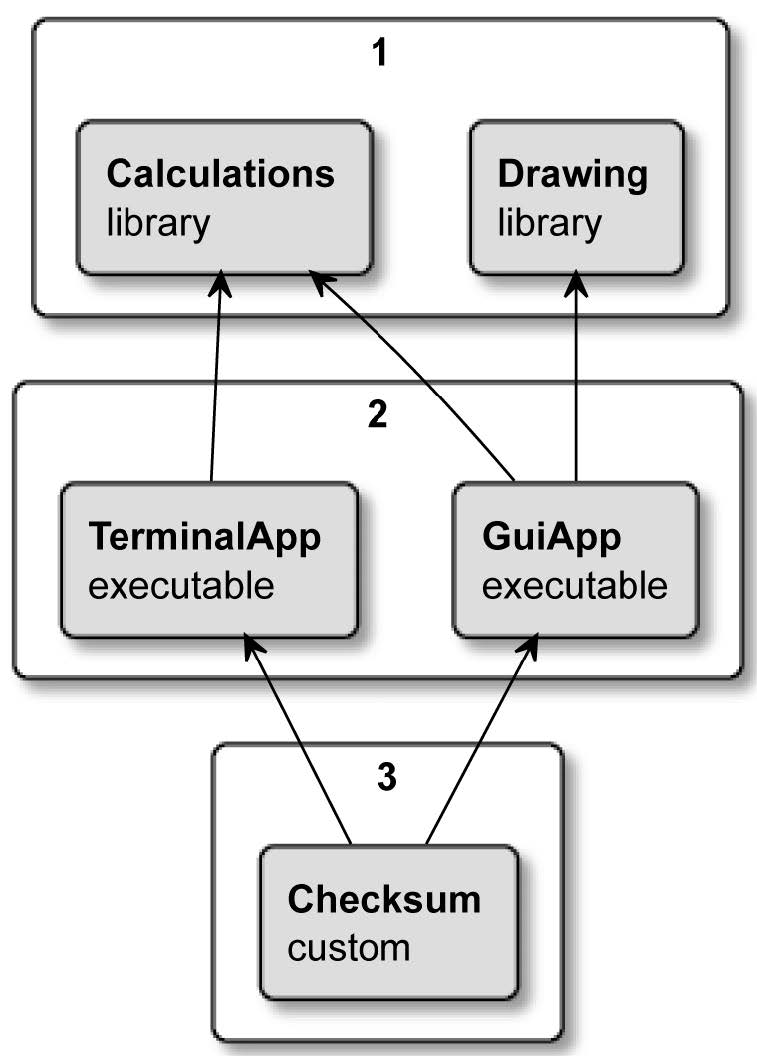
\includegraphics[width=0.4\textwidth]{content/2/chapter4/images/1.jpg}\\
图4.1  BankApp项目中构建依赖的顺序
\end{center}

这个项目中,有两个库、两个可执行程序和一个自定义目标。这里的用例是为用户提供一个银行应用,该应用程序具有一个漂亮的GUI(GuiApp),以及一个命令行版本,可作为自动化脚本(TerminalApp)的一部分使用。两个可执行程序都依赖于相同的计算库,但只有一个需要绘图库。为了确保应用程序下载正确,将计算一个校验和,将其存储在一个文件中,并通过单独的安全通道分发它。CMake在为这样的解决方案编写列表文件时非常灵活:

\begin{lstlisting}[style=styleCMake]
# chapter04/01-targets/CMakeLists.txt

cmake_minimum_required(VERSION 3.19.2)
project(BankApp CXX)

add_executable(terminal_app terminal_app.cpp)
add_executable(gui_app gui_app.cpp)

target_link_libraries(terminal_app calculations)
target_link_libraries(gui_app calculations drawing)

add_library(calculations calculations.cpp)
add_library(drawing drawing.cpp)

add_custom_target(checksum ALL
	COMMAND sh -c "cksum terminal_app>terminal.ck"
	COMMAND sh -c "cksum gui_app>gui.ck"
	BYPRODUCTS terminal.ck gui.ck
	COMMENT "Checking the sums..."
)
\end{lstlisting}

们使用target\_link\_libraries()指令将库与可执行文件连接起来。若没有它,可执行文件的编译将会因为未定义的符号而失败。我们在实际声明库之前调用了这个命令。当CMake配置项目时,其会收集关于目标,及其属性的信息——名称、依赖项、源文件和其他信息。

解析所有文件之后,CMake将尝试构建一个依赖图。和所有有效的依赖图一样,它们是有向无环图。有着一个明确的方向,确定哪个目标依赖于哪个目标,不过这样的依赖不能形成环。

当在构建模式下执行cmake时,生成的构建系统将检查我们已经定义的顶级目标并递归构建它们的依赖项。考虑一下图4.1中的例子:

\begin{enumerate}
\item 
从顶部开始,构建第1组中的两个库。

\item 
计算和绘图库完成后,构建组2 - GuiApp和TerminalApp。

\item 
构建一个校验和目标;运行指定的命令行生成校验和(cksum是一个Unix校验和工具)。
\end{enumerate}

有一个小问题——前面的解决方案并不能保证在可执行文件之后构建校验和目标。CMake不知道校验和依赖于当前的可执行二进制文件,所以可以自由地先开始构建它。为了解决这个问题,可以把add\_dependencies()指令放在文件的末尾:

\begin{lstlisting}[style=styleCMake]
add_dependencies(checksum terminal_app gui_app)
\end{lstlisting}

这将确保CMake理解Checksum目标和可执行程序之间的关系。

这很好,不过target\_link\_libraries()和add\_dependencies()之间有什么区别呢?第一个用于与实际库一起使用,并允许控制属性传播。第二种方法只能用于顶层目标,以设置它们的构建顺序。

随着项目变得越来越复杂,依赖树变得越来越难以理解。如何简化这个过程?

\subsubsubsection{4.2.2\hspace{0.2cm}可视化的依赖性}

即使是小项目也很有难和与其他开发人员直接分享。最简单的方法是通过一个漂亮的图表。毕竟,一张图片胜过千言万语。我们可以自己做这个工作并画一个图表,就像我在图4.1中所做的那样。但这很没意思,而且需要不断更新。幸运的是,CMake有一个很好的模块来生成点/graphviz格式的依赖关系图。它支持内部和外部依赖关系!

要使用它,可以简单地执行以下命令:

\begin{tcblisting}{commandshell={}}
cmake --graphviz=test.dot .
\end{tcblisting}

该模块将生成一个文本文件,可以将该文本文件导入Graphviz可视化软件,该软件可以渲染图像或生成PDF或SVG文件,这些文件可以作为软件文档的一部分存储。每个人都喜欢好的文档,但是几乎没有人喜欢创建文档——现在,不需要自己来做了!

如果你赶时间,甚至可以直接从浏览器运行Graphviz,地址如下:

\url{https://dreampuf.github.io/GraphvizOnline/}

\begin{tcolorbox}[colback=blue!5!white,colframe=blue!75!black,title=重要的Note]
自定义目标在默认情况下是不可见的,需要创建一个特殊的配置文件CMakeGraphVizOptions.cmake,它允许自定义图形。设置了一个方便的定制命令(GRAPHVIZ\_CUSTOM\_TARGETS TRUE);将其添加到特殊的配置文件中,以支持报告图中的自定义目标。可以在该模块的文档中找到更多选项。
\end{tcolorbox}

所需要做的就是复制和粘贴测试的内容。点文件到左边的窗口,项目将会可视化。很方便,不是吗?

\begin{center}
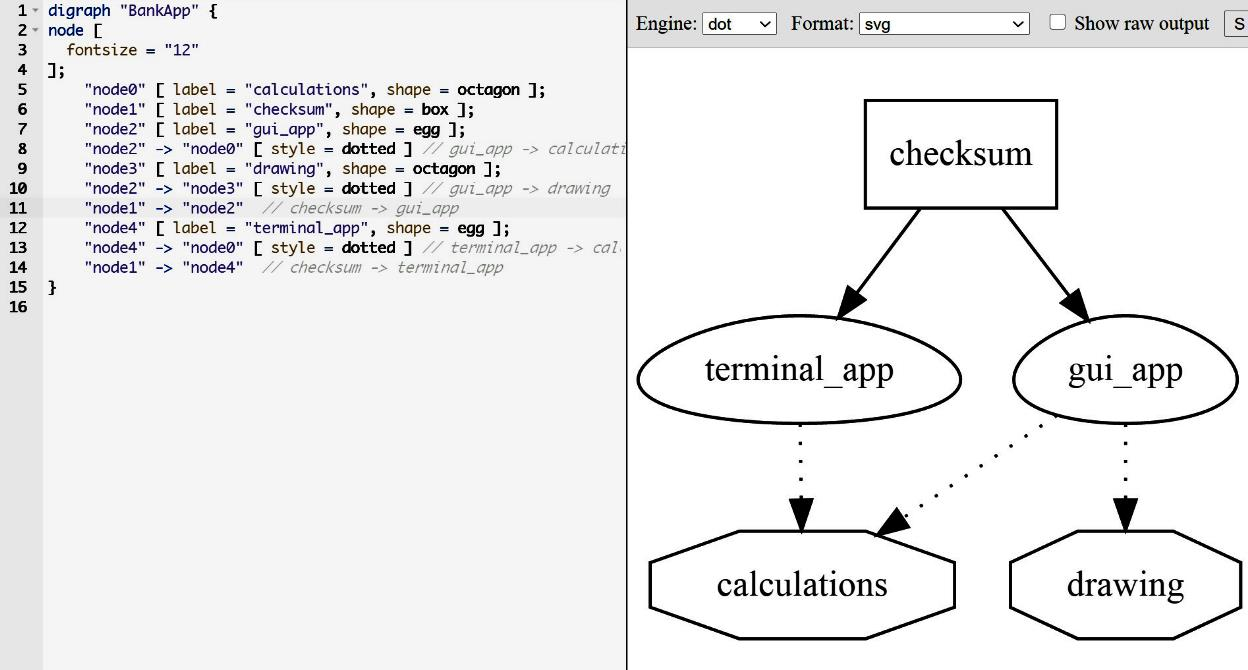
\includegraphics[width=0.8\textwidth]{content/2/chapter4/images/2.jpg}\\
图4.2  Graphviz中BankApp示例的可视化
\end{center}

为了清晰起见,从上图中删除了自动生成的图例部分。

使用这种方法,可以快速地看到所有显式定义的目标。现在有了这个全局视角,让我们深入研究一下如何配置。
 
\subsubsubsection{4.2.3\hspace{0.2cm}目标属性}

Targets have properties that work in a similar way to fields of C++ objects. We can modify some of these properties and others are read-only. CMake defines a large list of "known properties" (see the Further reading section) that are available depending on the type of the target (executable, library, or custom). You can also add your own properties if you like. Use the following commands to manipulate the properties of a target:

\begin{lstlisting}[style=styleCMake]
get_target_property(<var> <target> <property-name>)
set_target_properties(<target1> <target2> ...
						PROPERTIES <prop1-name> <value1>
						<prop2-name> <value2> ...)
\end{lstlisting}

To print a target property on screen, we first need to store it in the <var> variable and then message() it to the user; we have to read them one by one. On the other hand, setting properties on a target allows us to specify multiple properties at the same time, on multiple targets.

The concept of properties isn't unique to targets; CMake supports setting properties of other scopes as well: GLOBAL, DIRECTORY, SOURCE, INSTALL, TEST, and CACHE.

To manipulate all kinds of properties, there are general get\_property() and set\_property() commands. You can use these low-level commands to do exactly what the set\_target\_properties() command does, just with a bit more work:

\begin{lstlisting}[style=styleCMake]
set_property(TARGET <target> PROPERTY <name> <value>)
\end{lstlisting}

Generally, it's better to use as many high-level commands as you can. CMake offers more of these, even narrower in their scope, such as setting specific properties on a target. For example, add\_dependencies(<target> <dep>) is appending dependencies to the MANUALLY\_ADDED\_DEPENDENCIES target property. In this case, we can query it with get\_target\_property() exactly as with any other property. However, we can't use set\_target\_property() to change it (it's read-only), as CMake insists on using the add\_dependencies() command to restrict operations to appending only.

We'll introduce more property setting commands when we discuss compiling and linking in upcoming chapters. Meanwhile, let's focus on how the properties of one target can transition to another.

\subsubsubsection{4.2.4\hspace{0.2cm}可传递需求}

Let's just agree that naming is hard, and sometimes one ends up with a result that's hard to understand. "Transitive usage requirements" is, unfortunately, one of those cryptic titles that you will encounter in the online CMake documents. Let's untangle this strange name and perhaps propose a term easier to understand.

I'll start by clarifying the middle bit of this puzzle. As we previously discussed, one target may depend on another. CMake documentation sometimes refers to such dependency as usage, as in one target uses another. This was straightforward, so on to the next one.

There will be cases when such a used target has specific requirements that a using target has to meet: link some libraries, include a directory, or require specific compile features. All of these are in fact requirements, so documentation is correct in a sense. The issue is that they aren't called requirements in any other context in the documentation. When you specify the same requirements for a single target, you set properties or dependencies. Therefore, the last part of the name should perhaps be simply "properties."

The last part is –transitive. This one I believe is correct (maybe a bit too smart). CMake appends some properties/requirements of used targets to properties of targets using them. You can say that some properties can transition (or simply propagate) across targets implicitly, so it's easier to express dependencies.

Simplifying this whole concept, I see it as propagated properties between the source target (targets that gets used) and destination targets (targets that use other targets).

Let's look at a concrete example to understand why it's there and how it works:

\begin{lstlisting}[style=styleCMake]
target_compile_definitions(<source> <INTERFACE|PUBLIC|PRIVATE> 
	[items1...])
\end{lstlisting}

This target command will populate the COMPILE\_DEFINITIONS property of a <source> target. Compile definitions are simply -Dname=definition flags passed to the compiler that configure the C++ preprocessor definitions (we'll get to that in Chapter 5, Compiling C++ Sources with CMake). The interesting part here is the second argument. We need to specify one of three values, INTERFACE, PUBLIC, or PRIVATE, to control which targets the property should be passed to. Now, don't confuse these with C++ access specifiers – this is something else.

Propagation keywords work like this:

\begin{itemize}
\item 
PRIVATE sets the property of the source target.

\item 
INTERFACE sets the property of the destination targets.

\item 
PUBLIC sets the property of the source and destination targets.
\end{itemize}

When a property is not to be transitioned to any destination targets, set it to PRIVATE.
When such a transition is needed, go with PUBLIC. If you're in a situation where the source target doesn't use the property in its implementation (.cpp files) and only in headers, and these are passed to the consumer targets, INTERFACE is the answer.

How does this work under the hood? To manage those properties, CMake provides a few commands such as the aforementioned target\_compile\_definitions(). When you specify a PRIVATE or PUBLIC keyword, CMake will store provided values in the property of the target matching the command – in this case, COMPILE\_DEFINITIONS. Additionally, if a keyword was INTERFACE or PUBLIC, it will store the value in property with an INTERFACE\_ prefix – INTERFACE\_COMPILE\_DEFINITIONS. During the configuration stage, CMake will read the interface properties of source targets and append their contents to destination targets. There you have it – propagated properties, or transitive usage requirements – as CMake calls them.

In CMake 3.20, there are 12 such properties managed with appropriate commands such as target\_link\_options() or directly with the set\_target\_properties() command:

\begin{itemize}
\item 
AUTOUIC\_OPTIONS

\item 
COMPILE\_DEFINITIONS

\item 
COMPILE\_FEATURES

\item 
COMPILE\_OPTIONS

\item 
INCLUDE\_DIRECTORIES

\item 
LINK\_DEPENDS

\item 
LINK\_DIRECTORIES

\item 
LINK\_LIBRARIES

\item 
LINK\_OPTIONS

\item 
POSITION\_INDEPENDENT\_CODE

\item 
PRECOMPILE\_HEADERS

\item 
SOURCES
\end{itemize}

We'll discuss most of these options in the following pages, but remember that all of these options are, of course, described in the CMake manual. Find them on their own page under a URL in this format (replace <PROPERTY> with a property that interests you): 

\url{https://cmake.org/cmake/help/latest/prop_tgt/<PROPERTY>.html}

The next question that comes to mind is how far this propagation goes. Are the properties set just on the first destination target, or are they sent to the very top of the dependency graph? Actually, you get to decide.

To create a dependency between targets, we use the target\_link\_libraries() command. The full signature of this command requires a propagation keyword:

\begin{lstlisting}[style=styleCMake]
target_link_libraries(<target>
					<PRIVATE|PUBLIC|INTERFACE> <item>...
					[<PRIVATE|PUBLIC|INTERFACE> <item>...]...)
\end{lstlisting}

As you can see, this signature also specifies a propagation keyword, but this one controls where properties from the source target get stored in the destination target. Figure 4.3 shows what happens to a propagated property during the generation stage (after the configuration stage is completed):

\begin{center}
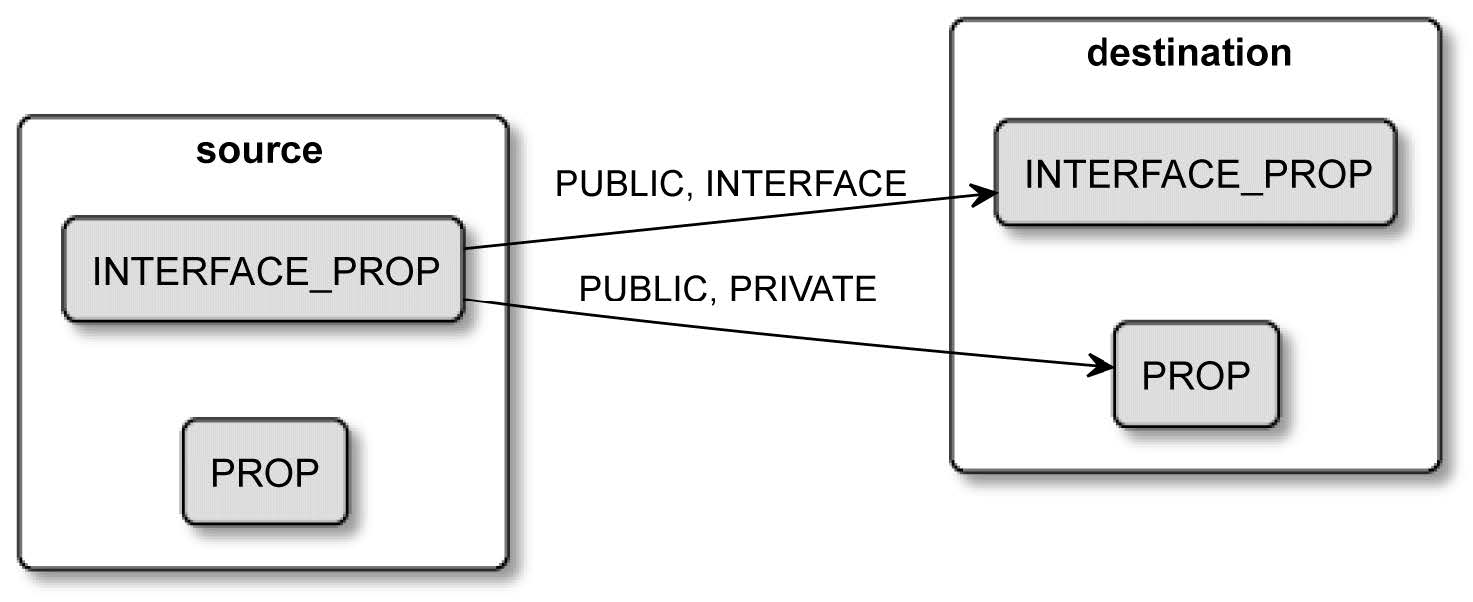
\includegraphics[width=0.8\textwidth]{content/2/chapter4/images/3.jpg}\\
Figure 4.3 – How properties are propagated to destination targets
\end{center}

Propagation keywords work like this:

\begin{itemize}
\item 
PRIVATE appends the source value to the private property of the destination.

\item 
INTERFACE appends the source value to the interface property of the destination.

\item 
PUBLIC appends to both properties of the destination.
\end{itemize}

As we discussed before, interface properties are only used to propagate the properties further down the chain, and the destination target won't use them in its build process.

The basic target\_link\_libraries(<target> <item>...) command that we used before implicitly specifies the PUBLIC keyword.

If you correctly set propagation keywords for your source targets, properties will be automatically placed on destination targets for you – unless there's a conflict…

\subsubsubsection{4.2.5\hspace{0.2cm}处理冲突的传播属性}

When one target depends on multiple other targets, there may be a situation where propagated properties are in outright conflict with each other. Say that one used target specifies the POSITION\_INDEPENDENT\_CODE property as true and the other as false. CMake understands this as a conflict and will print an error similar to this:

\begin{tcblisting}{commandshell={}}
CMake Error: The INTERFACE_POSITION_INDEPENDENT_CODE property
of "source_target2" does not agree with the value of POSITION_
INDEPENDENT_CODE already determined for "destination_target".
\end{tcblisting}

It is useful to receive such a message, as we explicitly know that we introduced this conflict and we need to resolve it. CMake has its own properties that have to "agree" between source and destination targets.

On rare occasions, this may become important – for example, if you're building software using the same library in multiple targets that are then linked to a single executable. If these source targets are using different versions of the same library, you may run into problems.

To make sure that we're only using the same specific version, we can create a custom interface property, INTERFACE\_LIB\_VERSION, and store the version there. This is not enough to solve the problem, as CMake won't propagate custom properties by default. We have to explicitly add a custom property to a list of "compatible" properties.

Each target has four such lists:

\begin{itemize}
\item 
COMPATIBLE\_INTERFACE\_BOOL

\item 
COMPATIBLE\_INTERFACE\_STRING

\item 
COMPATIBLE\_INTERFACE\_NUMBER\_MAX

\item 
COMPATIBLE\_INTERFACE\_NUMBER\_MIN
\end{itemize}

Appending your property to one of them will trigger propagation and compatibility checks. The BOOL list will check whether all properties propagated to the destination target evaluate to the same Boolean value. Analogically, STRING will evaluate to a string. NUMBER\_MAX and NUMBER\_MIN are a bit different – propagated values don't have to match, but the destination target will just receive the highest or the lowest value instead.

This example will help us to understand how to apply this in practice:

\begin{lstlisting}[style=styleCMake]
# chapter04/02-propagated/CMakeLists.txt

cmake_minimum_required(VERSION 3.20.0)
project(PropagatedProperties CXX)

add_library(source1 empty.cpp)
set_property(TARGET source1 PROPERTY INTERFACE_LIB_VERSION
	4)
set_property(TARGET source1 APPEND PROPERTY
	COMPATIBLE_INTERFACE_STRING LIB_VERSION
)
add_library(source2 empty.cpp)

set_property(TARGET source2 PROPERTY INTERFACE_LIB_VERSION
	4)
add_library(destination empty.cpp)
target_link_libraries(destination source1 source2)
\end{lstlisting}

We create three targets here; for simplicity, all are using the same empty source file. On both of the source targets, we specify our custom property with the INTERFACE\_ prefix. And we set them to the same matching library version. Both of the source targets are linked to the destination target. Finally, we specify a STRING compatibility requirement as a property for source1 (we don't add the INTERFACE\_ prefix here).

CMake will propagate this custom property to the destination target and check whether the version of all the source targets is an exact match (the compatibility property can be set on just one target).

Now that we understand what targets are, let's take a look at other things that look like targets, smell like targets, and sometimes act like targets but, as it turns out, aren't the real deal.

\subsubsubsection{4.2.6\hspace{0.2cm}实现伪目标}

The concept of a target is so useful that it would be great if some of its behaviors could be borrowed for other things too. This is, specifically, things that do not represent outputs of the buildsystem but rather inputs – external dependencies, aliases, and so on. These are the pseudo targets, or targets that don't make it to the generated buildsystem.

\hspace*{\fill} \\ %插入空行
\noindent
\textbf{导入目标}

If you skimmed the table of contents, you know that we'll be talking about how CMake manages external dependencies – other projects, libraries, and so on. IMPORTED targets are essentially products of this process. CMake can define them as a result of the find\_ package() command.

You can adjust the target properties of such a target: compile definitions, compile options, include directories, and so on – and they will even support transitive usage requirements. However, you should treat them as immutable; don't change their sources or dependencies.

The scope of the definition of an IMPORTED target can be global or local to the directory where it was defined (visible in subdirectories but not in parent directories).

\hspace*{\fill} \\ %插入空行
\noindent
\textbf{别名目标}

Alias targets do exactly what you expect – they create another reference to a target under a different name. You can create alias targets for executables and libraries with the following commands:

\begin{lstlisting}[style=styleCMake]
add_executable(<name> ALIAS <target>)
add_library(<name> ALIAS <target>)
\end{lstlisting}

Properties of alias targets are read-only, and you cannot install or export aliases (they aren't visible in the generated buildsystem).

So, what is the reason to have aliases at all? They come in handy in scenarios where some part of a project (such as a subdirectory) requires a target with a specific name, and the actual implementation may be available under different names depending on circumstances. For example, you may wish to build a library shipped with your solution or import it based on a user's choice.

\hspace*{\fill} \\ %插入空行
\noindent
\textbf{接口库}

This is an interesting construct – a library that doesn't compile anything but instead serves as a utility target. Its whole concept is built around propagated properties (transitive usage requirements).

Interface libraries have two primary uses – to represent header-only libraries and to bundle a bunch of propagated properties into a single logical unit.

Header-only libraries are fairly easy to create with add\_library(INTERFACE):

\begin{lstlisting}[style=styleCMake]
add_library(Eigen INTERFACE
	src/eigen.h src/vector.h src/matrix.h
)
target_include_directories(Eigen INTERFACE
	$<BUILD_INTERFACE:${CMAKE_CURRENT_SOURCE_DIR}/src>
	$<INSTALL_INTERFACE:include/Eigen>
)
\end{lstlisting}

In the preceding snippet, we created an Eigen interface library with three headers. Next, with generator expressions (explained in the last section of this chapter), we set its include directories to be \$\{CMAKE\_CURRENT\_SOURCE\_DIR\}/src when a target is exported and include/Eigen when it's installed (which will also be explained at the end of this chapter).

To use such a library, we just have to link it:

\begin{lstlisting}[style=styleCMake]
target_link_libraries(executable Eigen)
\end{lstlisting}

No actual linking occurs here, but CMake will understand this command as a request to propagate all the INTERFACE properties to the executable target.

The second use case leverages exactly the same mechanism but for a different purpose – it creates a logical target that can be a placeholder for propagated properties. We can then use this target as a dependency for other targets and set properties in a clean, convenient way. Here's an example:

\begin{lstlisting}[style=styleCMake]
add_library(warning_props INTERFACE)
target_compile_options(warning_props INTERFACE
	-Wall -Wextra -Wpedantic
)
target_link_libraries(executable warning_props)
\end{lstlisting}

The add\_library(INTERFACE) command creates a logical warning\_props target that is used to set compile options specified in the second command on the executable target. I recommend using these INTERFACE targets, as they improve the readability and reusability of your code. Think of it as refactoring a bunch of magic values to a wellnamed variable. I also suggest using the \_props suffix to easily differentiate interface libraries from the regular ones.

Are pseudo targets exhausting the concept of the target? Of course not! That would simply be too easy. We still need to understand how these targets translate to produced buildsystems.

\subsubsubsection{4.2.7\hspace{0.2cm}构建目标}

Target is a bit of a loaded word. It means different things in the context of a project and the context of generated buildsystems. When CMake generates a buildsystem, it "compiles" list files from CMake language to the language of a chosen build tool; perhaps it creates a Makefile for GNU Make. Such Makefiles have their own targets – some of them are direct conversions of list file targets, and others are created implicitly.

One such buildsystem target is ALL, which CMake generates by default to contain all top-level list file targets, such as executables and libraries (not necessarily custom targets). ALL is built when we run cmake -{}-build <build tree> without choosing a concrete target. As you might remember from the first chapter, you can choose one by adding the -{}-target <name> parameter to the preceding command.

Some executables or libraries might not be needed in every build, but we'd like to keep them as part of the project for those rare occasions when they come in useful. To optimize our default build, we can exclude them from the ALL target like so:

\begin{lstlisting}[style=styleCMake]
add_executable(<name> EXCLUDE_FROM_ALL [<source>...])
add_library(<name> EXCLUDE_FROM_ALL [<source>...])
\end{lstlisting}

Custom targets work the other way around – by default, they're excluded from the ALL target unless you explicitly define them with an ALL keyword, as we did in the BankApp example.

Another implicitly defined build target is clean, which simply removes produced artifacts from the build tree. We use it to get rid of all old files and build everything from scratch. It's important though to understand that it don't just simply delete everything in the build directory. This means that for clean to work correctly, you need to manually specify any files that your custom targets might create as BYPRODUCTS (see the BankApp example).

There's also an interesting non-target mechanism to create custom artifacts that can be used in all actual targets – custom commands.

